% introduction.tex
% Narrative structure:
% (1) motivation, stylized facts, and multi-asset requirements;
% (2) strengths and limitations of existing single-asset generators;
% (3) strengths and limitations of multi-asset dependence models;
% (4) study question, approach, main evidence, and scope.

Researchers and practitioners often use synthetic paths to stress-test risk
models against unobserved market scenarios, validate portfolio
optimization algorithms, and evaluate allocation strategies across
many simulations~\cite{assefaEtAl2020, jordonEtAl2022}.
However, synthetic financial data often fail to capture important statistical
features of real returns~\cite{stengerEtAl2024}. Daily excess growth
rates for a broad-market exchange-traded fund (ticker SPY)
from $2014$--$2024$ illustrate three widely documented stylized
facts~\cite{mandelbrot1963, cont2001}
(Fig.~\ref{fig:empirical_motivation}). Most observed
returns lie close to zero, but extreme returns occur much more often
than a Gaussian model predicts
(Fig.~\ref{fig:empirical_motivation}a and
Fig.~\ref{fig:empirical_motivation}b). Raw growth rates show little
correlation across days (Fig.~\ref{fig:empirical_motivation}c). Absolute
growth rates, in contrast, remain positively correlated over
longer periods (Fig.~\ref{fig:empirical_motivation}d), so large and
small changes cluster over time. Matching the marginal return distribution
alone therefore does not reproduce how volatility evolves over time.
Multi-asset simulations must also reproduce cross-asset dependence to
evaluate portfolio risk and performance under different rebalancing
strategies~\cite{embrechtsMcNeilStraumann2002, boucheyNemtchinovWong2015}.
Building a multi-asset simulation therefore starts with choosing a single-asset
generator that reproduces each asset's return distribution and volatility
dynamics.

\begin{figure}[tbp]
    \centering
    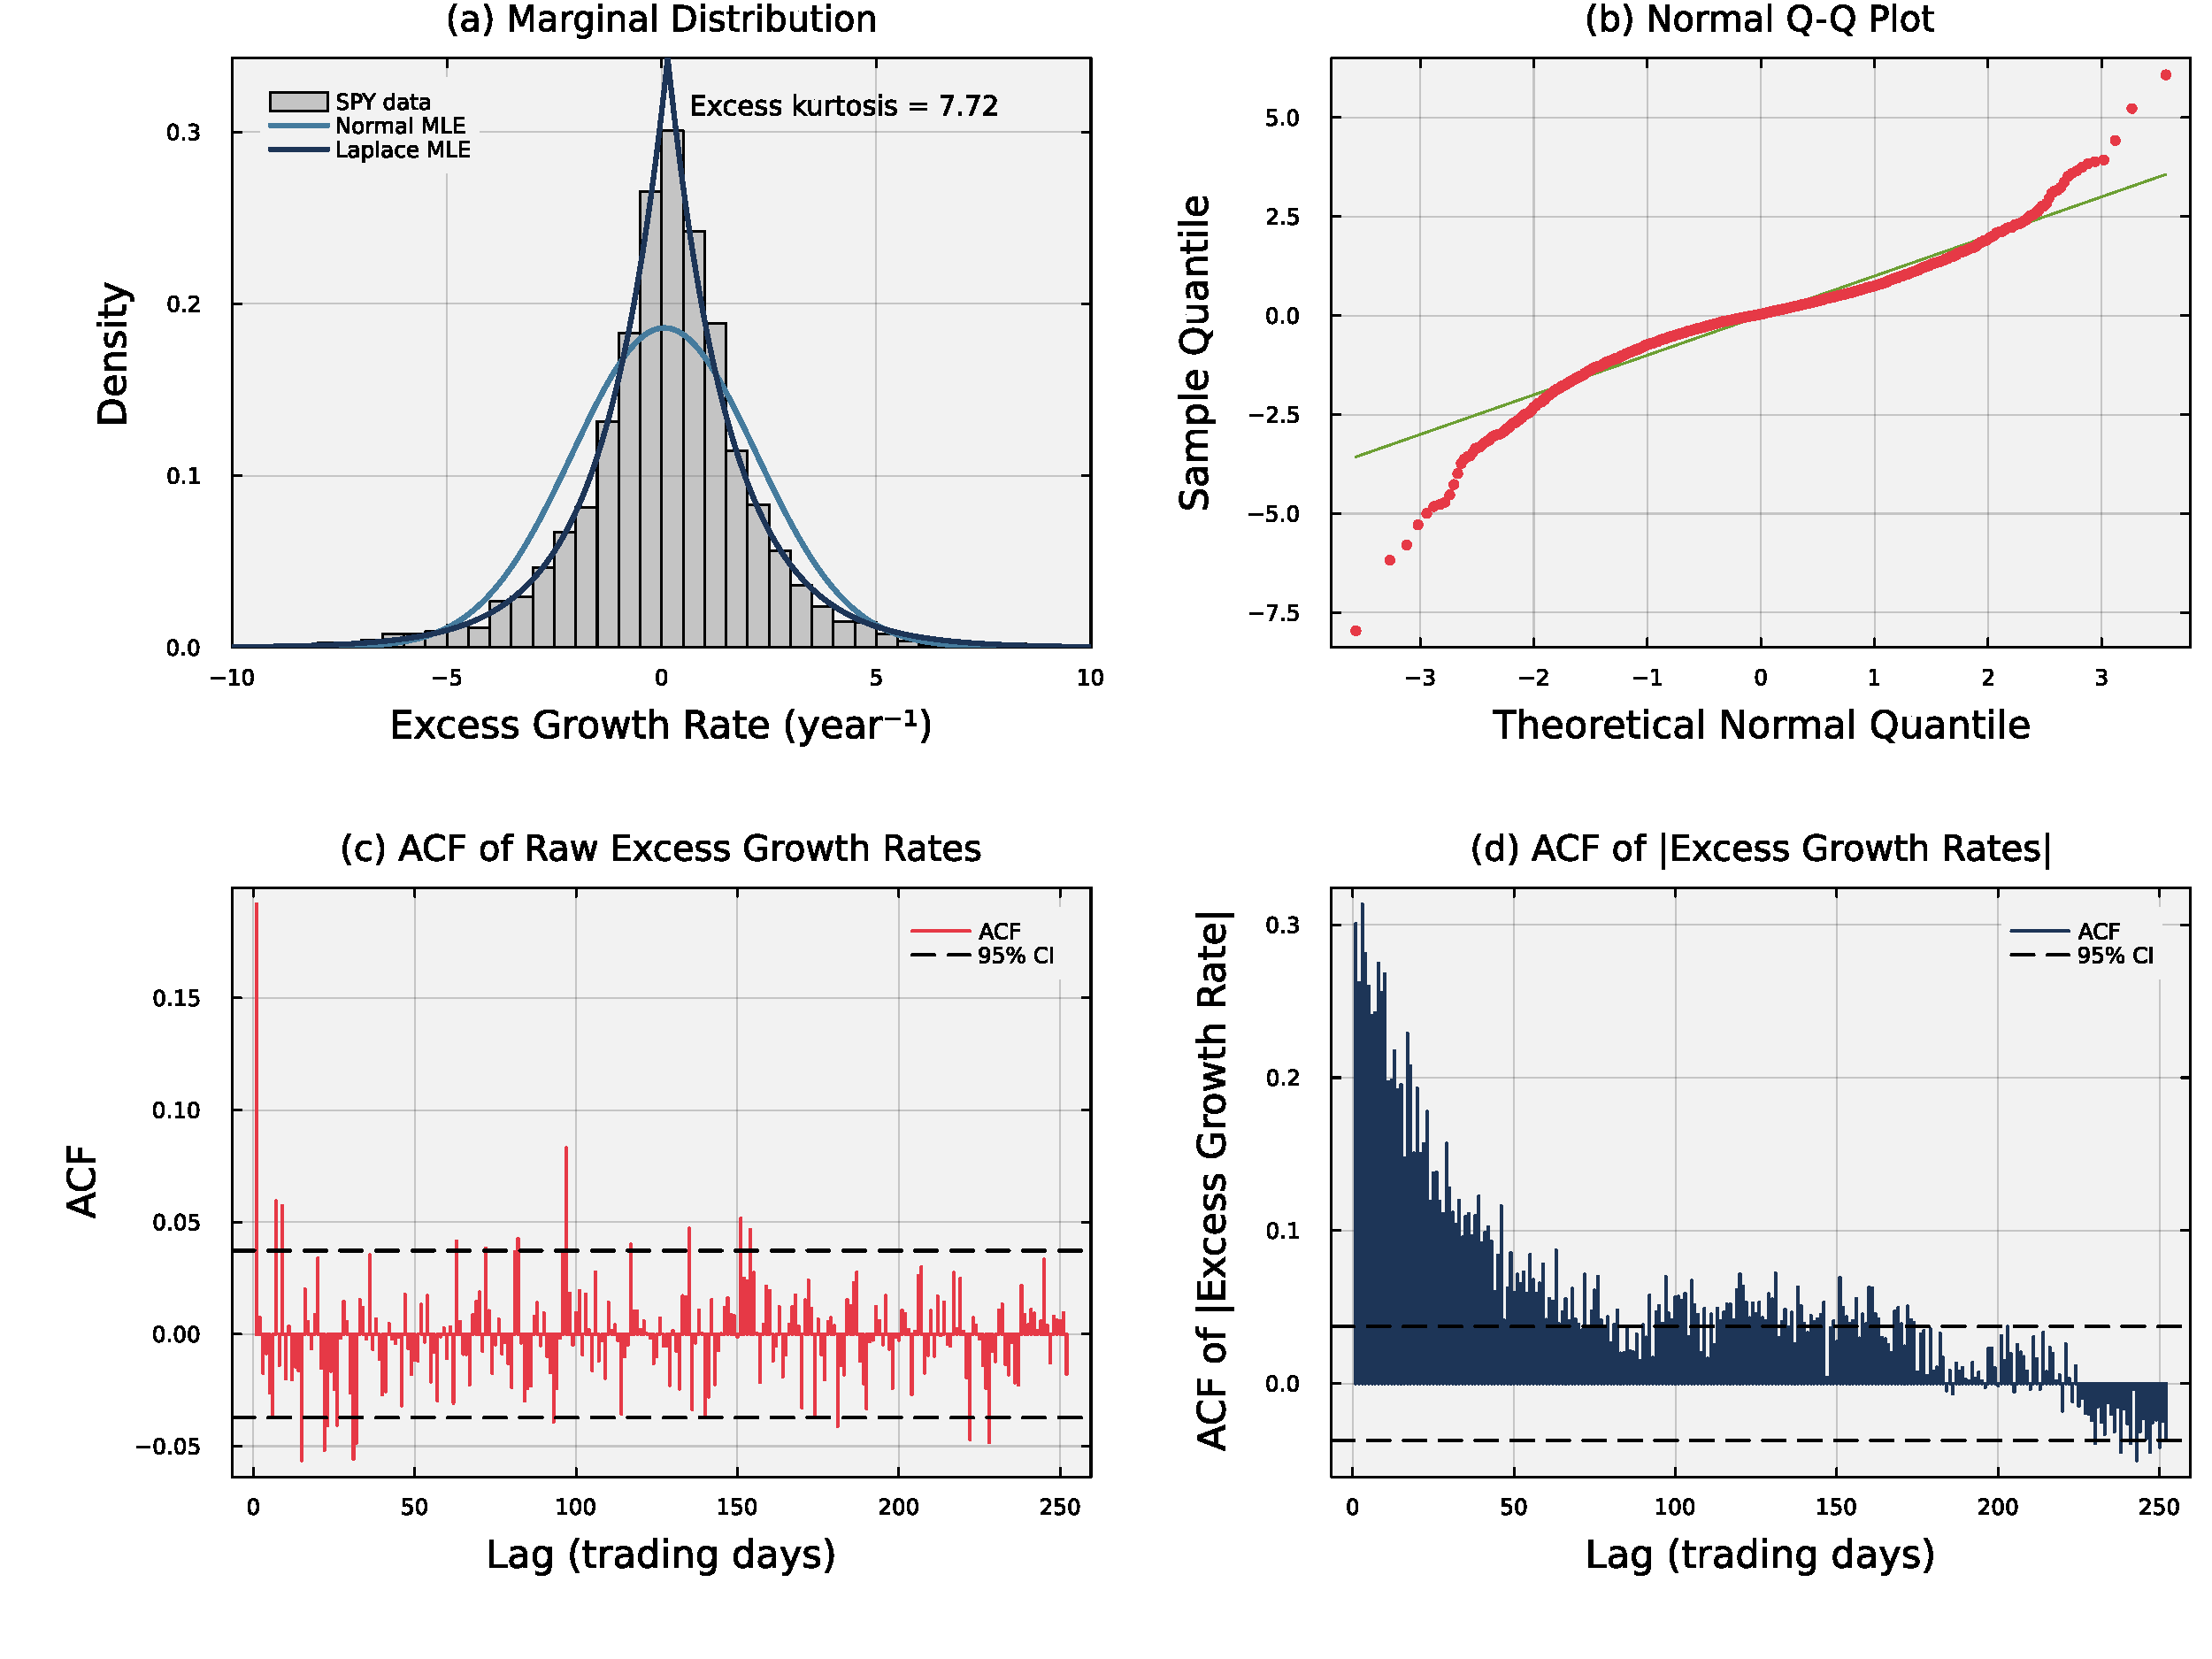
\includegraphics[width=\textwidth]{figs/main/Fig01-Empirical-Motivation.pdf}
    \caption{\textbf{Empirical stylized facts of SPY daily excess growth
    rates ($2014$--$2024$).} Panel~(a) shows the heavy-tailed return
    density; the Laplace maximum-likelihood fit tracks the empirical
    peak and tails while the Gaussian fit does not. Panel~(b) shows
    departure from the diagonal in a normal quantile-quantile plot
    at both extremes. Panel~(c) shows the
    autocorrelation function of raw excess growth rates. Individual
    correlations are small, although the Ljung--Box test detects joint
    serial dependence. Panel~(d) shows the autocorrelation function
    of absolute excess growth rates, which decays slowly across the
    reported lags.}
    \label{fig:empirical_motivation}
\end{figure}

Single-asset generators differ in the return features they reproduce and in
the effort required to fit them across a large asset universe. Generalized
autoregressive conditional heteroskedasticity (GARCH) models
capture volatility clustering, but may require heavy-tailed innovations to
reproduce extreme returns~\cite{engle1982, bollerslev1986}.
Stochastic-volatility models represent persistent changes in volatility,
while jump-diffusion models represent abrupt
extremes~\cite{heston1993, merton1976, kou2002}. Jumps alone do not produce
persistent volatility. Deep generative models can learn flexible return
distributions and temporal patterns. Some generative adversarial networks
(GANs) reproduce volatility
clustering and other path-dependent features~\cite{wieseEtAl2020,niEtAl2021}.
Other evaluations of GANs and the time-series generative adversarial
network (TimeGAN) miss the absolute-return autocorrelation
associated with volatility clustering~\cite{takahashiEtAl2019,
yoonEtAl2019timegan,kwonLee2024}. Hidden Markov models provide interpretable
market regimes, but
standard transition rules can leave high-volatility states too quickly to
reproduce long clusters of large returns~\cite{rabinerJuang1986,
rydenTerasvirtaAsbrink1998, bullaBulla2006}. Choosing a single-asset model
requires balancing distributional fit, volatility persistence,
interpretability, and the effort required to fit the model across hundreds of
assets. Portfolio simulation adds a separate requirement because independently
fitted single-asset models do not specify how assets move together.

Multivariate hidden-state models allow assets to share market
regimes, but become harder to fit as the number of assets
grows~\cite{diasVermuntRamos2010}. Copula models combine separately fitted
asset distributions with a model of cross-asset dependence and can capture
nonlinear and tail relationships~\cite{embrechtsMcNeilStraumann2002,
cherubiniLucianoVecchiato2004, aasCzadoFrigessiBakken2009}. However, copula
models require choosing a dependence structure, and standard static copulas do
not describe how dependence changes across days. Factor models are easier to
apply to large asset universes because each asset is linked to a small number
of shared factors instead of modeling every relationship between pairs of
assets~\cite{sharpe1963, rossAPT1976, famaFrench1993}. The single-index model
separates each asset's return into a market component and an asset-specific
residual. After fitting the model, the historical residuals are easy to
calculate. The residuals can be resampled or used to fit a separate generator
for each asset. Fitting residual generators is a direct solution, but adds a
second fitting step for every asset. Generating residual paths independently
also misses sector, style, and other relationships not explained by the
market. Reusing an existing full-return generator avoids the second fit and
preserves the fitted return distribution and temporal behavior. However, a
full-return draw already contains the asset mean and market-related variance.
Treating the full-return draw as a residual can shift the mean and count market
variance twice. The problem is not how to calculate residuals. The problem is
whether an existing full-return generator can be reused without shifting the
mean or inflating the variance. Dependence among the residuals remains a
separate problem.

In this study, we explored how to build a multi-asset generator from
separately fitted single-asset components and a shared market path without
shifting expected returns or overcounting market variance. We used a
hidden Markov model (HMM) for each asset, with Laplace-quantile states,
Student-$t$ emissions, and counted transitions. Temporary episodes in the
extreme states distinguished the hidden Markov model with jumps
(\mbox{HMM-WJ}) from the hidden Markov model with no jumps (\mbox{HMM-NJ}). On a decade
of SPY data, HMM-WJ reduced absolute-return autocorrelation error
relative to HMM-NJ while retaining a high in-sample
Kolmogorov--Smirnov pass rate. GARCH achieved a lower autocorrelation
error but did not match the return distribution, so HMM-WJ served as a
practical per-asset generator rather than a uniformly superior model. For
multi-asset composition, we centered and rescaled each asset-level path before
adding a shared SPY path. The correction removed the mean shift and prevented
the market contribution to variance from being counted twice without fitting
another model to each asset's regression residuals. We tested the correction
on $423$ non-market assets in a $424$-asset universe and set the jump
probability to zero to isolate the composition rule. With all $2014$--$2024$
parameters held fixed, the correction increased the mean Kolmogorov--Smirnov
pass rate across $416$ complete asset histories from
$2025$ and brought the median ratio of synthetic to observed variance
from inflated under naive composition to near one. Independent residual generation did not reproduce residual
dependence and could overstate returns from daily rebalancing.
